\section{Problem Definition}\label{sec:prelims}
The {\probname} defines a generating process that creates new items, at each step, and distributes copies of these items between different sets of nodes:

\begin{definition}[Generating Process]
Let $U=\set{1,\ldots,n}$ be a set of nodes, $\F$ a family of subsets of $U$, and $\pi:\F \rightarrow [0,1]$. 
A \emph{generating process} $\sys = (U, \F,\pi)$ is an infinite time process that at each time $t$, generates a collection of subsets $\S_t \subseteq\F$, such that a set $S\in \F$ is included in the sample $\S_t$  with probability $\pi(S)$, independent of other sets. 
An \emph{item} $i_{t,S}$ is a \emph{copy} of $S\in\F$ generated at time $t$, and thus, $i_{t,S}\in \S_t$.
% Each node is a set $S\in \S_t$ receives a copy of a new item  $i_{t,S}$.
%Thus, $\sys$ generates a sequence $\S_1,\S_2,\ldots$ where each $\S_t$ is a sample of {\ins}s generated at time $t$. An \emph{item} $i_{t,S}$ is a \emph{copy} of the {\ins} $\S$ generated at time $t$.
We call the elements of $\F$ \emph{\ins} of $U$.
\end{definition}

A probing schedule is a probability distribution over the possible sets of nodes to probe in each step. Note that we are interested in efficient \emph{memoryless} schedules that can be stored and computed efficiently.

\begin{definition}[Schedule]
A \emph{$c$-schedule}, for a positive integer $c$, is a probability distribution $\p$ over $U$ such that at any time step, the schedule probes (up to) $c$ nodes independently chosen according to the distribution $\p$. We say an item $i_{t,S}$ is \emph{caught} at time $t'\geq t$, if $\p$ probes a node of $S$ at time $t'$, and no node of $S$ was probed in the interval $[t,t'-1]$.
\end{definition}
% \begin{definition}[Schedule]
% A \emph{$c$-schedule}, for a positive integer $c$, is a probability distribution $\p$ over $U^c$ such that at any time step, the schedule probes (up to) $c$ nodes chosen according to the distribution $\p$. We say an item $i_{t,S}$ is \emph{caught} at time $t'\geq t$, if $\p$ probes a node of $\S$ at time $t'$, and no node of $S$ was probed in the interval $[t'-1,t]$.
% \end{definition}
For simplicity, we may say schedule instead of $c$-schedule if it is clear in the context. 
The cost of a schedule is the expected number of undetected items at a given step, weighted by their freshness, and averaged over time:
\begin{definition}[$\theta$-Cost]
Let $\theta\in(0,1]$ be a decaying factor. The \emph{freshness} of an \emph{uncaught} item $i_{t,S}$ at time $t'\geq t$ is $\theta^{t'-t}$. The \emph{load} of $\sys$ at time $t$, denoted by $L_\sys(t)$, is the sum of the freshness of uncaught items at time $t$. The $\theta$-\emph{cost}, or \emph{cost} in short, of a schedule $\p$ is defined as 
$\lim\limits_{t\rightarrow\infty}\frac{1}{t}\sum_{t'=0}^{t}\E(L_\sys(t'))$. 
We denote the cost of $\p$ by $\cost{\p}$.
% = \sum_{S\in\F}\frac{\pi(S)}{1-\theta(1-\p(S))}.$$
\end{definition} 
Thus, the cost function is the limit expected load of the system, averaged over time. Note that this limit always exists as proven in Lemma~\ref{lem:explicit}. 
% There is always a schedule with finite cost (e.g. the uniform random distribution). 
Our goal is to compute a schedule with minimum cost:
% \ahmad{Therefore, the cost function is the \emph{expected} load of the system, averaged over the time.}
% Our goal is to compute a schedule with minimum cost:
\begin{definition}[\probname]
 The goal in a $(\theta,c)$-{\probname}, or $(\theta,c)$-PHSP, for a generating system $\sys$ is to find  a $c$-schedule with the minimum $\theta$-cost. We call a schedule \emph{optimal} if it has the minimum cost.
\end{definition}

Note that in $(\theta,c)$-PHSP, the parameter $\theta$ tunes our interest in older items. For instance, if $\theta$ is close to 0, an ideal schedule should catch as many \emph{new items} (generated in very recent time steps) as possible.
% (\ahmad{This can be viewed as a multi-arm bandit problem where each element $u\in U$ represents a bandit, and the score we get total freshness of the items that we catch by probing $u$})
 In the other extreme, if $\theta=1$, an ideal schedule should consider all the items for catching, regardless of their age.

% then each item will stay in the system only for one step as its freshness disappears immediately. So, ideally, a schedule should catch as many \emph{new items} (generated in the current time step) as possible 

In other words, an ideal schedule for a $(\theta, c)$-PHSP is a schedule that spends more time on probing the nodes that are more likely to receive ``fresh'' items: if the items are the ``information'' that flow over the network, these nodes play the role of  \emph{information hubs} among the nodes. Our search for information hubs can be view as the complement of the ``influence maximization problem''\cite{Kempe2003,Kempe2005}. In the influence maximization we look for a set of nodes that generate the information that reach most nodes. In the information hubs problem we are looking for the set of nodes that receive the most amount of information, thus the most informative nodes.


% \subsection{Further Applications}
% Although we introduced the $(\theta,c)$-PHSP as a network search and detection problem, it defines a general probing framework with further applications, in particular in the study of social network properties, such as finding the most \emph{influential}~\cite{borgs2014maximizing,kempe} or the most \emph{central}~\cite{yoshida2014almost} set of nodes:
 

% \paragraph {\bf Influence Maximization:} Given a social social network $G=(U,E)$ and a cascade model for propagation on $G$, the goal is to find a set of $c$ nodes that maximizes the size of the cascade seeded at these nodes. In \cite{borgs2014maximizing} they introduced the notation of random hyper-edge, a random subset of nodes sampled according to a distribution $\pi'$. They showed that for a given set of nodes $N$, the influence of $N$, $\sigma(N)$, is
%  \begin{equation}\label{eq:infmax}
% \sigma(N) = n\cdot \pr_{S\sim \pi'} (N \cap S \neq \emptyset),
%  \end{equation}
%  where $n$ is the number of nodes in $G$. Thus, a set $N\subseteq U$ of size $c$ has the maximum influence if and only if it maximizes $\Pr_{S\sim \pi'}(N\cap S\neq \emptyset)$. 
%  
%  Now, let $\sys=(U,\F,\pi)$ be the generating system in which $\F$ is the family of all subsets of $U$ and $\forall S\in \F: \ \pi(S) = \pi'(S)$. Suppose $\p$ is an optimal $c$-schedule of the $(0,c)$-PHSP for $\sys$. Note that without loss of generality, since $\theta=0$, we can assume that $\p$ always  probes a \emph{fixed} set of $c$ nodes, $N$, that minimizes the total missing freshness, i.e., the total probability of the items that $\p$ does not catch at a time step; this is because after each step all the items are removed and the system resets. So, we have
%  $$\cost{\p} = \min_{N'\subseteq U: |N'|=c} 1 - \Pr_{S\sim \pi'}(N'\cap S\neq \emptyset) = 1 - \Pr_{S\sim \pi'}(N\cap S\neq \emptyset),$$
%  and thus, $\Pr_{S\sim \pi'}(N\cap S\neq \emptyset)$ is maximized and $N$ is a set of $c$ nodes with maximum influence. 
%  Therefore, the Influence Maximization problem can be translated into a proper $(0,c)$-PHSP.
%  
%  
%  \paragraph {\bf Set Centrality Maximization\cite{yoshida2014almost}:} 
%  In~\cite{yoshida2014almost} the problem of finding a set of $c$ nodes with maximum centrality was studied, for two different centrality measures (betweenness and coverage). Here, we see how finding a set (of size $c$) with maximum betweenness centrality can be presented as a $(0,c)$-PHSP (the results hold for coverage centrality as well using the proper hyper-edges introduced in~\cite{yoshida2014almost}).
%  
%  In a network $G=(U,E)$, the betweenness centrality of a set $N\subseteq U$ is defined as\footnote{In some other works, different normalizing factors are considered. However, without loss of generality we let the normalizing factor to be $\frac{1}{n(n-1)}$.}
%  $$C(N) = \frac{1}{n(n-1)}\sum_{u,v\in V} \frac{\tau(u,v; N)}{\tau(u,v)}$$
%  where $\tau(u,v)$ is the number of shortest path from $u$ to $v$, and $\tau(u,v;N)$ is the number of shortest path from $u$ to $v$ that pass any node in $N$. The goal is to find a set of $c$ nodes with maximum betweenness centrality. Suppose $\pi'$ is a distribution over the shortest paths of $G$, where each shortest path $P_{u,v}$ is chosen with probability $\frac{1}{n(n-1)\tau(u,v)}$. If $\texttt{in}(P)$ denotes the internal nodes of the path $P$, it has been shown~\cite{yoshida2014almost,mattoe?} the most central set of $c$ nodes is a set $N$ such that 
%  $$N\in \argmax_{N'\subseteq U: |N'|=c} \pr_{P\in\pi'}(\texttt{in}(P)\cap N' \neq \emptyset).$$
%  
%  
% Let $\F$ be the family of sets $S$ where each $S$ is the internal nodes of a shortest path in $G$, and define 
%  $$\forall S\in\F : \ \pi(S)=\sum_{\text{shortest path} P: \texttt{in}(P)=S} \pi'(S).$$
% Now, if $\sys=(U,\F,\pi)$ is a generating system, using a similar argument as above, we can assume that an optimal $c$-schedule for its $(0,c)$-PHSP probes a fixed set of $c$ nodes, $N$, that also has the maximum centrality.
% %\end{itemize}
% 
% % Obviously, the $c$-PHSP is an NP-hard problem as it reduces to other NP-hard problems (e.g., influence maximization). However, these reductions are to the cases where $\theta=0$ and general positive integer $c$. 
% In this work, we focus on $(\theta,1)$-PHSPs. In the following sections, we first study the $(\theta,1)$-PHSPs and provide different methods for finding the optimal schedule. We also show how in a generating system $\sys=(U,\F,\pi)$ our method works even if we do not have access to $\F$ or $\pi$, using only the samples of {\ins}s generated by $\sys$. Next, we show the scalablity of our method in using the MapReduce framework. Finally, we apply our method to a variety of real networks, and the results of our experiments demonstrate the practicality and optimality of our solution. 




% $\theta \in (0,1)$ and $c=1$ (see Figure~\ref{fig:square}) and show that it is possible to find  an optimal probing schedule for $1$-PHSP in $\sys=(\F, \pi, \theta)$, efficiently, and without having any prior information on distribution of items, i.e., knowing $\pi$ is not assumed in our algorithm.


% \begin{figure}[h!]
%   \centering
%     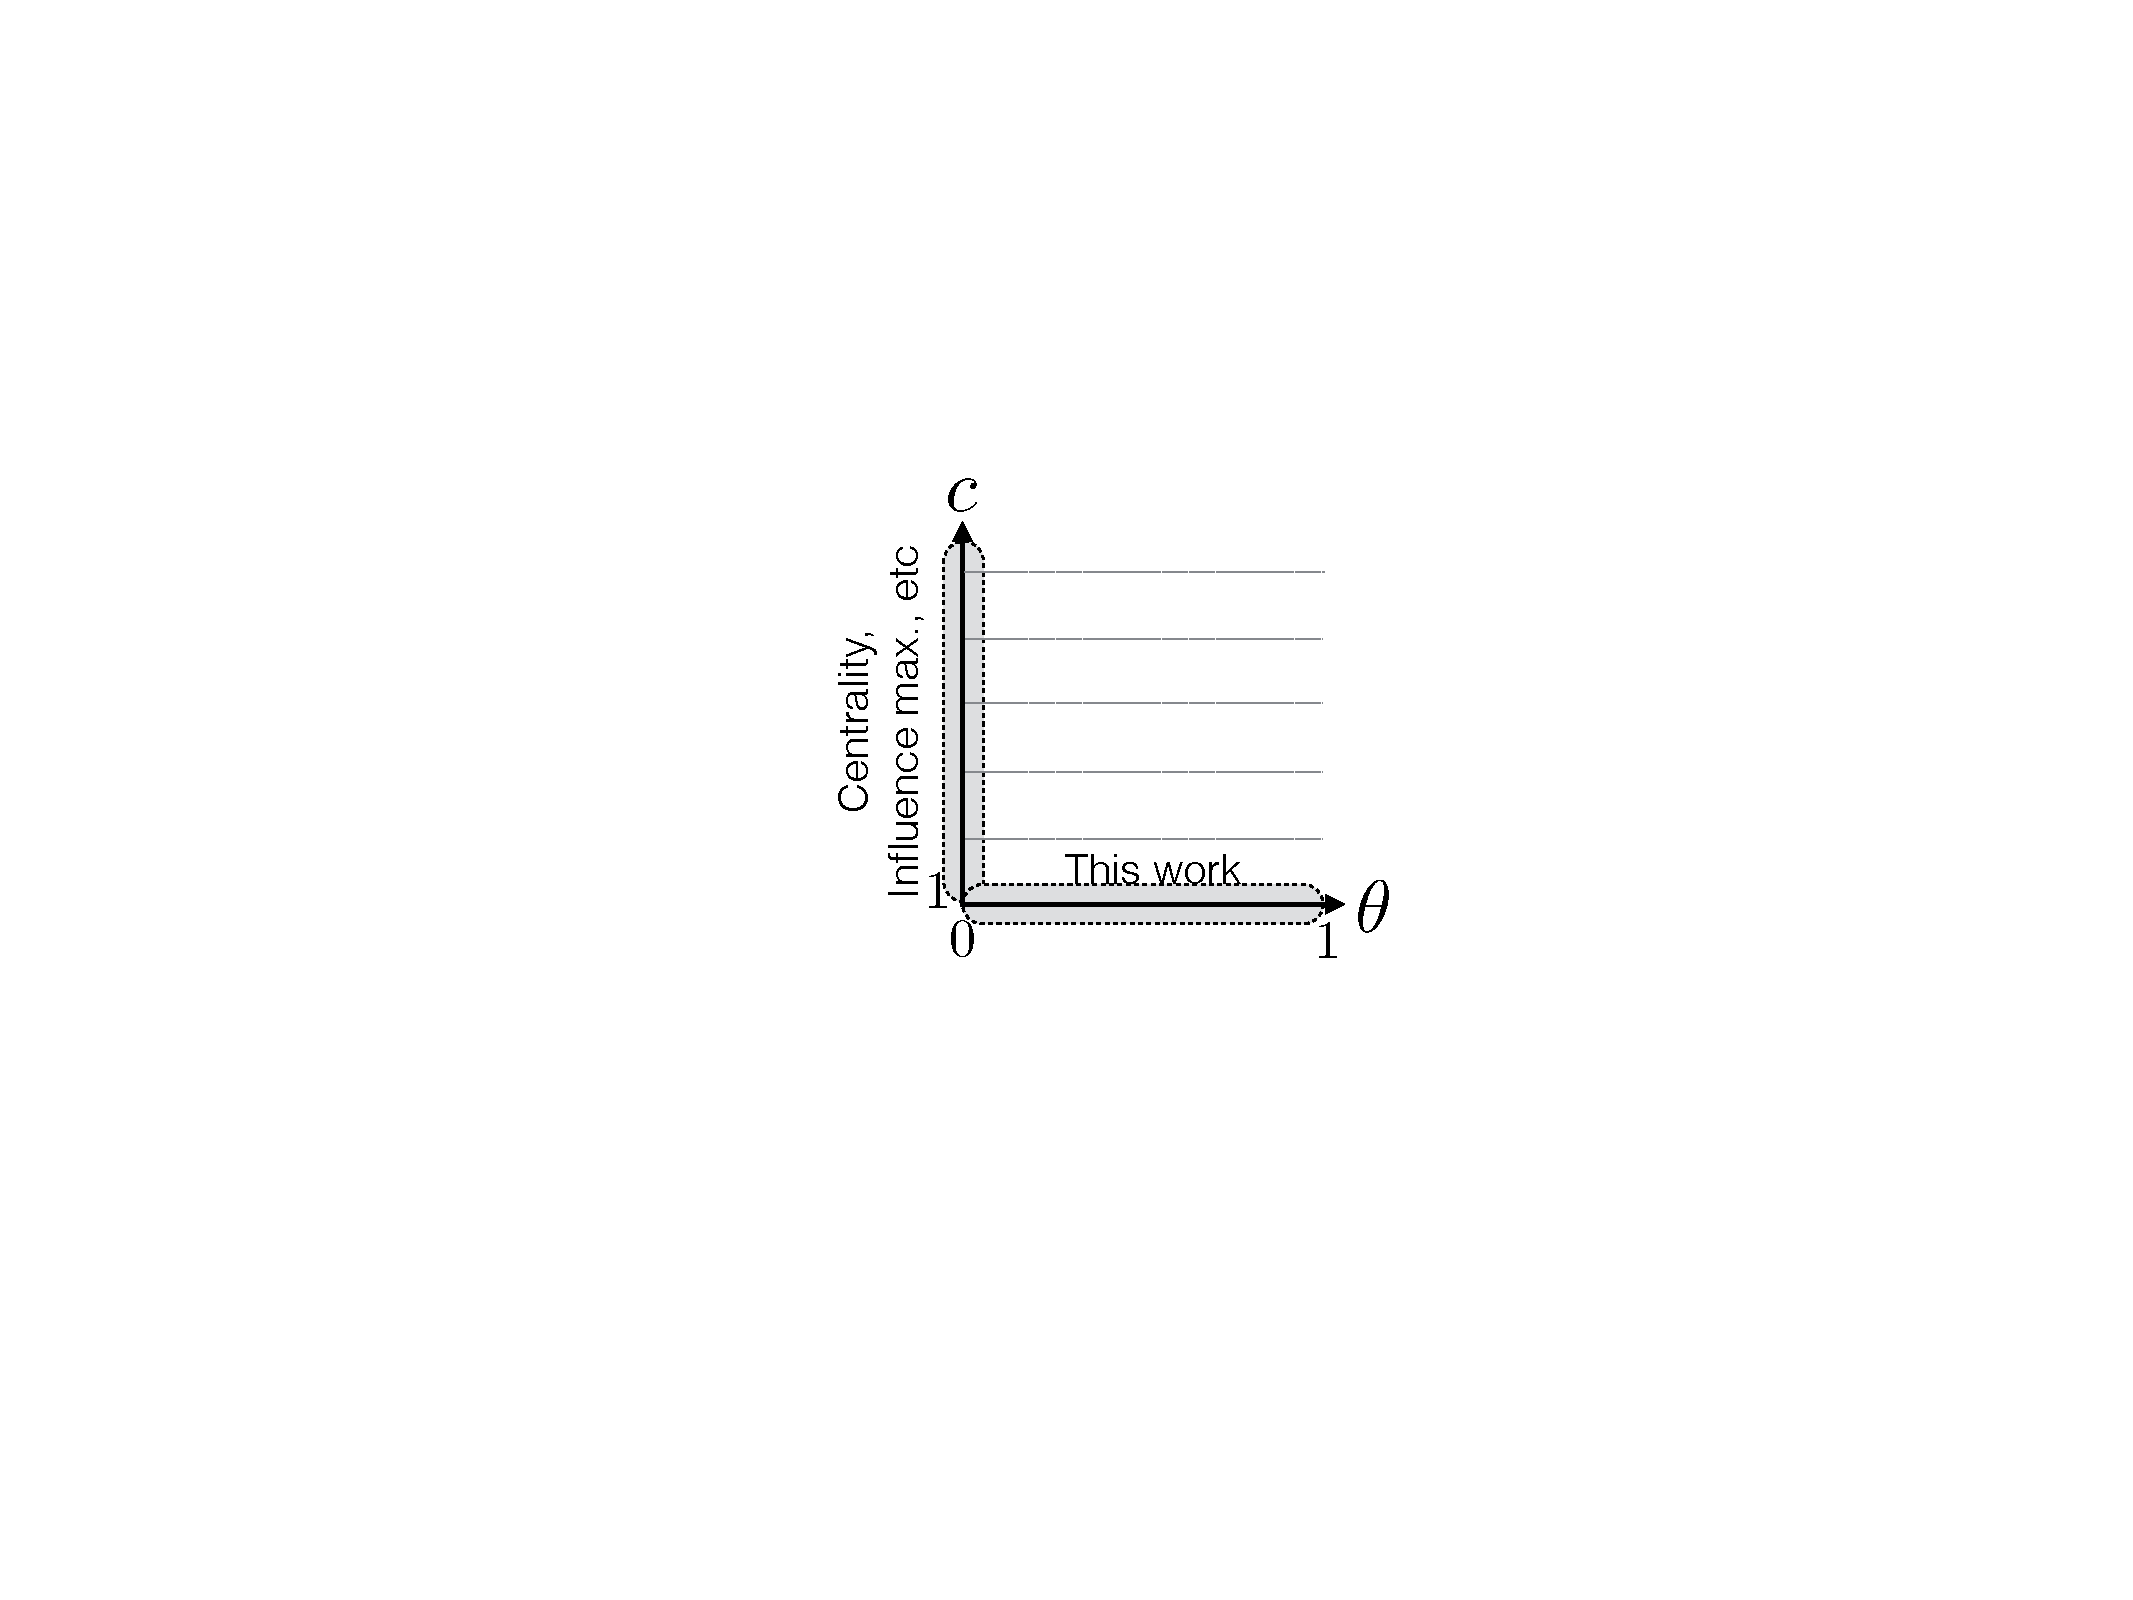
\includegraphics[width=0.25\textwidth]{figures/square.pdf}
%  \caption{}
% \label{fig:square}
% \end{figure}



